\section{Experimental Evaluation}

This section aims to answer the following research questions: 

\begin{itemize}
\item \textbf{Performance:} How is \NM{}'s performance on synthetic benchmarks and real applications, comparing to popular allocators and NUMA-aware allocators? (Section~\ref{sec:performance}) 
\item \textbf{Memory Consumption:} What is the memory consumption of \NM{}? (Section~\ref{sec:memory})
\item \textbf{Scalability:} How is the scalability of \NM{}? (Section~\ref{sec:scale})
\item \textbf{Design Decisions:} How important design choices can actually affect the performance? (Section~\ref{sec:design})	
\end{itemize}

\subsection{Experimental Setup}
\begin{table}[h]
  \footnotesize
  \setlength{\tabcolsep}{1.0em}
\begin{tabular}{c c c}
\hline
System & \textbf{Machine A} & \textbf{Machine B} \\ \hline
CPUs/Model & Xeon Gold 6138	& \\ \hline
NUMA Nodes & 2 & 8 \\ \hline
Physical Cores & 2$\times$20 & 8$\times$16 \\ \hline
Node Latency & \specialcell{local: 1.0 \\ 1 hop: 2.1} & \\ \hline
Interconnect Bandwidth & 8GT/s & \\ \hline
Memory Bandwidth & 19.87 GB/s & \\ \hline
  \end{tabular}
  \centering
  \caption{Machine Specifications.\label{table:Machine}}
\end{table}


Hardware platform:

Software (OS), Compiler: 

\subsection{Performance Evaluation}

\label{sec:performance}


We compare \NM{} with multiple popular allocators, such as Linux's glibc allocator, TcMalloc~\cite{tcmalloc}, or NUMA Aware TcMalloc~\cite{tcmallocnew}, jemalloc~\cite{jemalloc}, Scalloc~\cite{Scalloc}. For the simplicity, NUMA aware TcMalloc is called as TcMalloc-NUMA in the remainder of this paper. 

Performance evaluation will be performed on two different hardware as further described in the Table~\ref{table:Machine}:

%numactl --hardware Finding out latency information across nodes. 
% numactl --show Will show the physical core id information. 




%Scalloc is located in https://github.com/cksystemsgroup/scalloc

% Christoph also has a benchmark suite to evaluate the performance of memory allocator. 

% export LD_LIBRARY_PATH="/usr/local/lib/" for running tcmalloc.


%\paragraph{Application Statistics} We also checked the corresponding details of \\
\subsubsection{Synthetic Applications}
\label{sec:synthetic}

To make our evaluation results more convincing, we evaluated 23 applications, and showed both normalized values for every single of them and final average normalized values in the following sections. All the values are normalized based on the performance results of Linux's glibc allocator, so that a smaller value less than one means better performance and vice versa. Among the 23 applications, twelve are from the PARSEC suite~\cite{parsec} of applications, seven are real applications like Apache httpd-2.4.35, MySQL-5.7.15, Memcached-1.4.25, SQLite-3.12.0, Aget, Pfscan, and Pbzip2, and rest four are benchmarks from Hoard~\cite{Hoard}, including threadtest, larson, active-false sharing and passive-false sharing. All of these benchmarks are multi-threaded application and threads are distributed over nodes in our target machines sharing data with each other more or less, which made them more relevant toward gauging performance on modern NUMA machines than single-threaded benchmark suites, such as SPEC.

\subsubsection{Real Applications}
\label{sec:synthetic}

The number of threads of all benchmarks were adjusted according how many cores and nodes in the target machine to make threads could be properly distributed over the nodes and cores, making the number of threads as close as the number of cores. Mostly, thread number was 40 in the Machine A and 128 in the Machine B, and I will give the specific number below if it is not this default value. For specific, in PARSEC applications, native inputs~\cite{parsec} were used here.For MySQL, we used sysbench with 16 threads and 100,000 max requests. Besides, python-memcached~\cite{memcached} script was used for memcached with 3000 loops to get sufficient runtime and ab~\cite{apachetest} is used to test Apache by sending 1,000,000 requests. For Aget, we tested it by dowloading a 30 M file. For Pfscan, we executed a keyword search in a 500M data. In terms of Pbzip2, we tested it by compressing 10 30M files. Finally, SQLite was tested through a program called "threadtest3.c"~\cite{sqlitetest}. In the Hoard~\cite{Hoard} benchmarks, we used 100 iterations and 1,280,000 64-byte objects for threadtest and also we run larson for 10 seconds with 1,000 7-2048 bytes object to cover all size classes in almost all allocators for 10,000 iterations.For false sharing , we used 100,000 inner-loop , 100,000 iterations with 8 bytes objects. 

\begin{figure}[H]
    \centering
    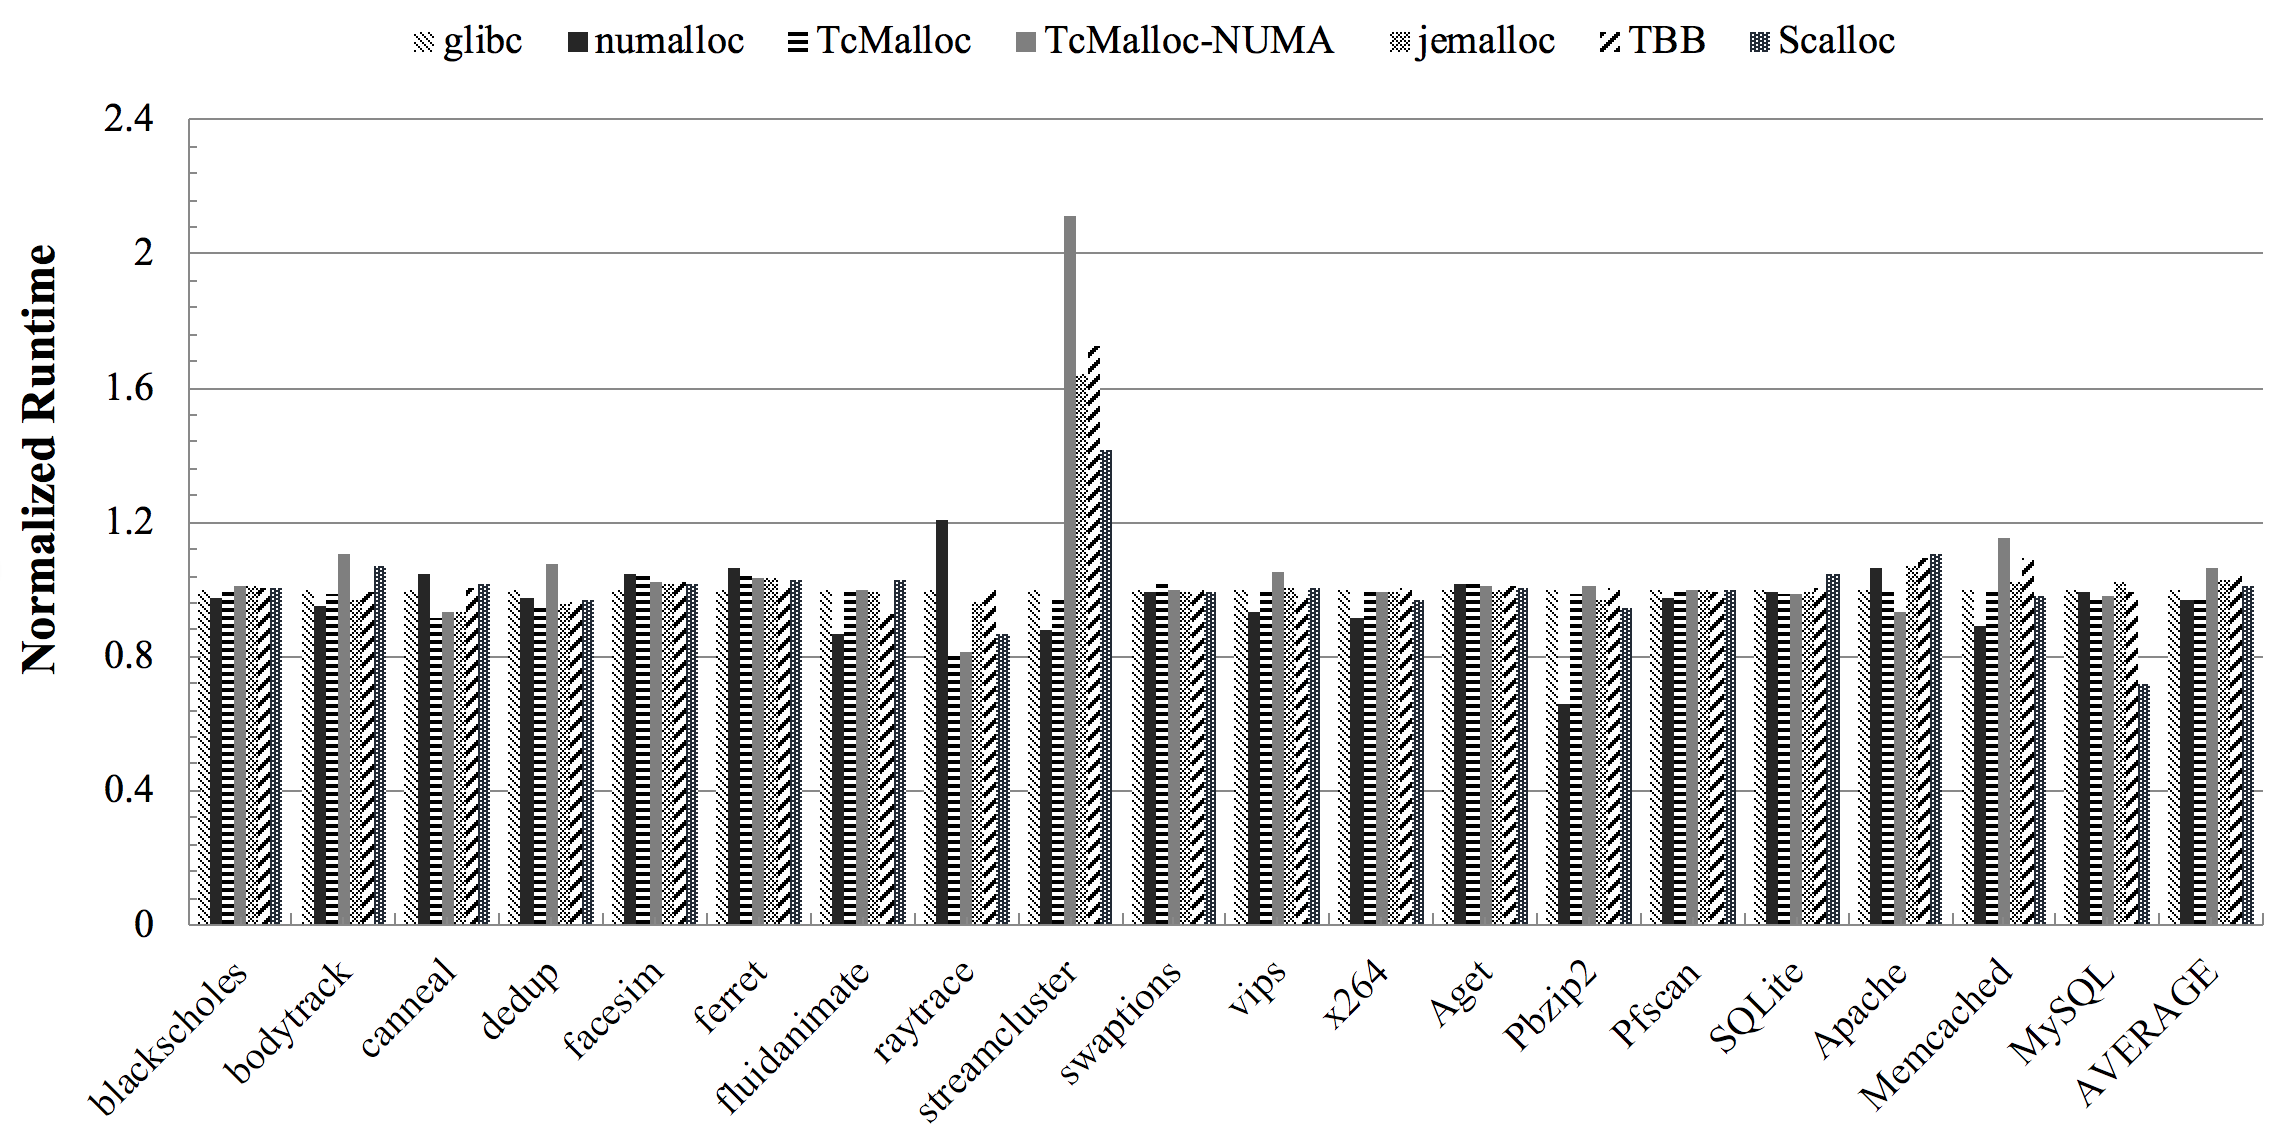
\includegraphics[width=\textwidth,height=200]{figure/2-node-parsec-perf.png}
    \caption{Normalized runtime with different allocators for PARSEC and real applications in Machine A}
    \label{2node-parsec-perf}
\end{figure}

\begin{figure}[H]
    \centering
    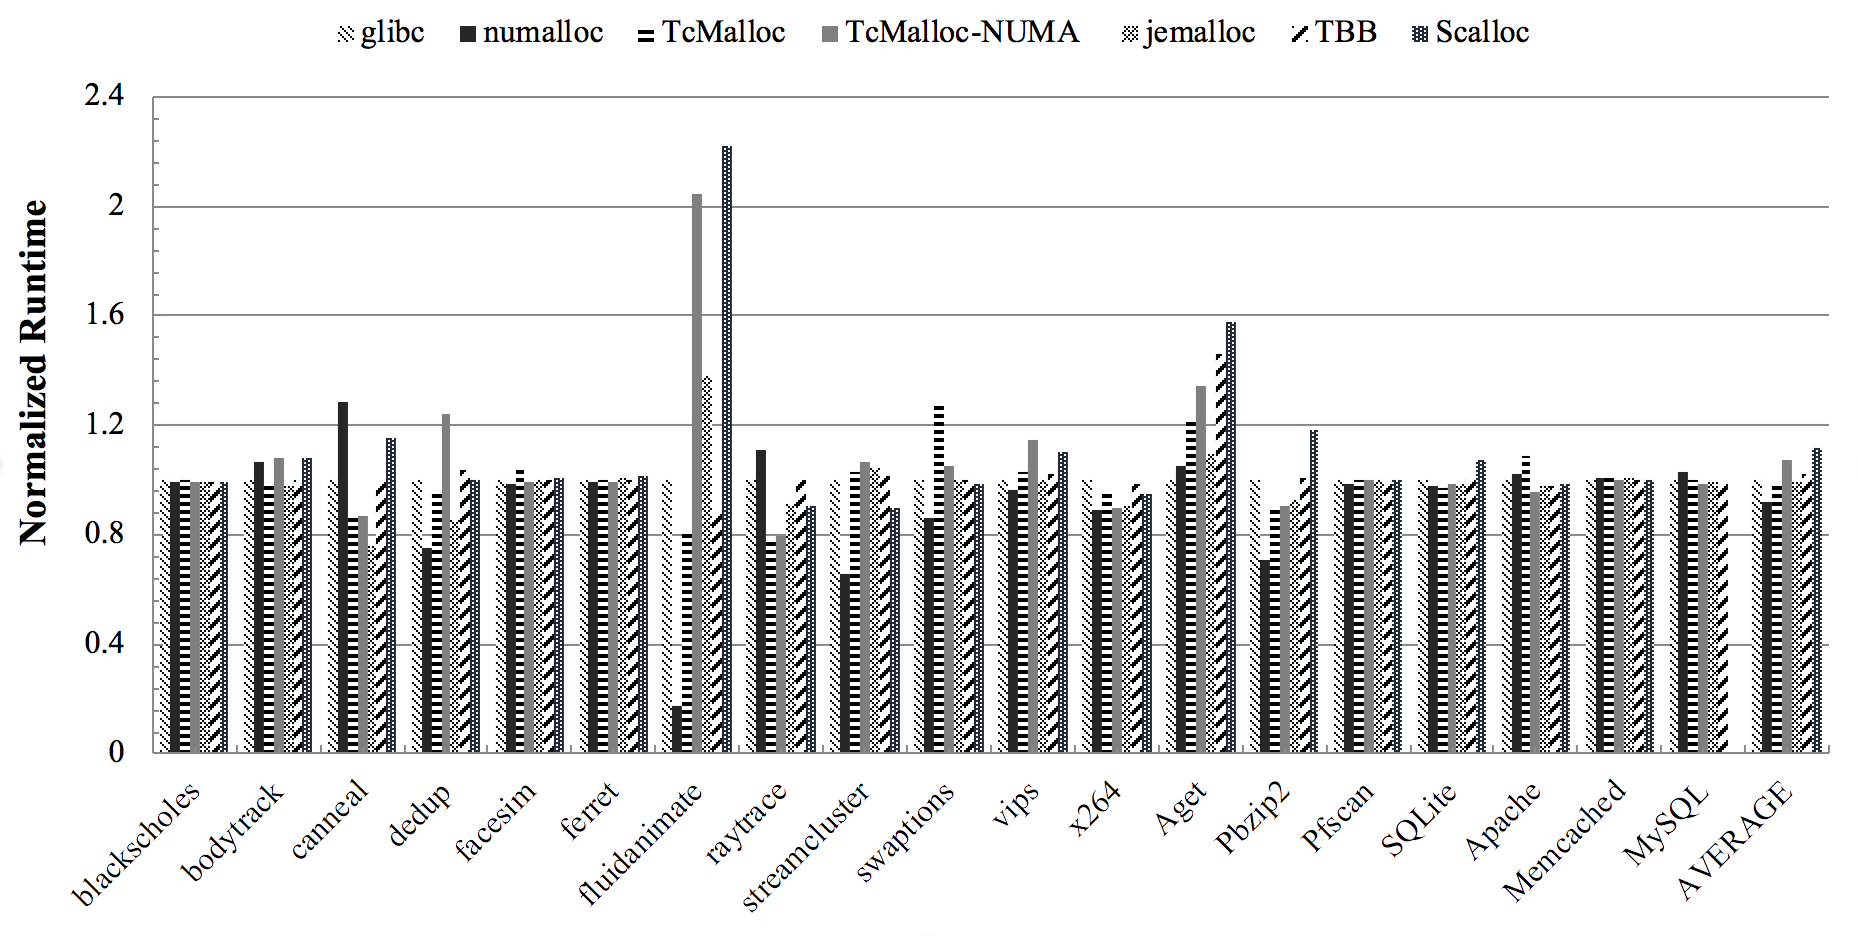
\includegraphics[width=\textwidth,height=200]{figure/8-node-parsec-perf.png}
    \caption{Normalized runtime with different allocators for PARSEC and real applications in Machine B}
    \label{8node-parsec-perf}
\end{figure}

Figure ~\ref{2node-parsec-perf} shows the normalized runtime of different allocators in Machine A and figure ~\ref{8node-parsec-perf} is for Machine B, compared with Linux allocator. We can see that the average value of \NM{} is 0.97 in Machine A and 0.92 in Machine B and it is always the best among all other allocators. The reason that \NM{} got better performance in Machine B is that there are more nodes and more cores in Machine B, which means \NM{} could be very helpful to better to take use hardware resource of multi nodes and cores.In the figure ~\ref{2node-parsec-perf}, we could get that the average normalized performance of \NM{} is 0.97 that is the best through these 7 allocators with 0.98 for TcMalloc, 1.00 for Scalloc. And \NM{} is also the best for most of single applications here, especially for fluidanimate, streamcluster and x264 in which 10 percent of improvements or even more are gotten. Besides \NM{}'s performance of  ratrace and canneal is not very good here, which is caused by their few data sharing between threads, but we could get amazing improvement if we shutdown interleaved heap in \NM{} and we will give the data in following sections.In the figure ~\ref{8node-parsec-perf}, we could see more exciting improvement from \NM{}, with average normalized value of 0.92 that is not only the best but also far aware better than all the rest allocators that TcMalloc and jemalloc got 0.99, TcMalloc-NUMA and TBB got roughly 1.07 and 1.01 separately. And also, we can see that the performance of \NM{} is the best for almost each single applications, especially it got 0.17 in fluidanimate and 0.66 in streamcluster which is far better than any of other allocators. As the same thing, the performance of ratrace and canneal is not good here, we will talk about it later after we shut down the interleaved heap.

\begin{figure}[H]
    \centering
    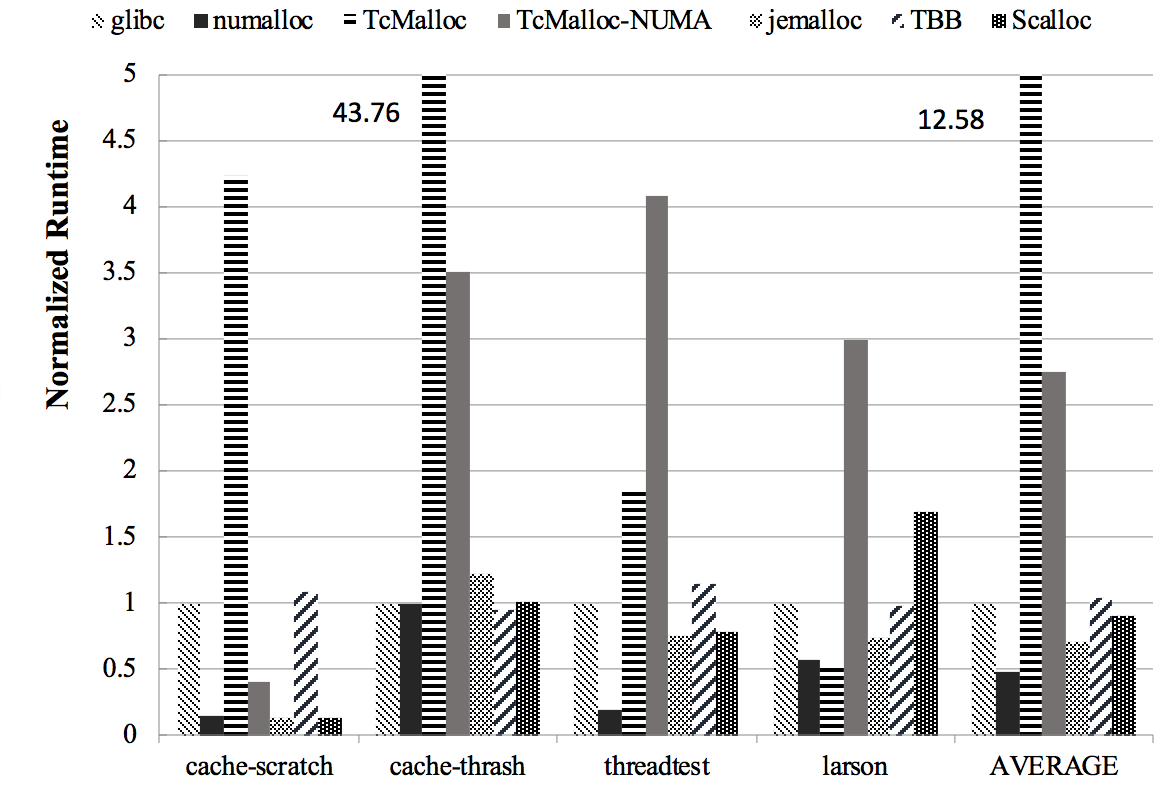
\includegraphics[width=\textwidth,height=200]{figure/2-node-hoard-perf.png}
    \caption{Normalized runtime with different allocators for Hoard benchmarks in Machine A}
    \label{2node-hoard-perf}
\end{figure}

\begin{figure}[H]
    \centering
    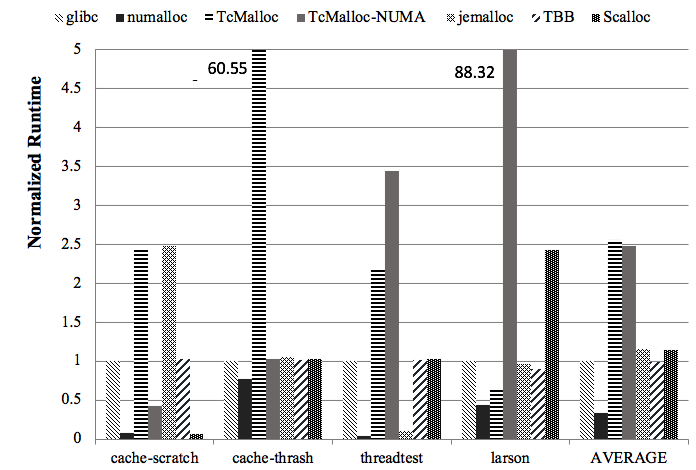
\includegraphics[width=\textwidth,height=200]{figure/8-node-hoard-perf.png}
    \caption{Normalized runtime with different allocators for Hoard benchmarks in Machine B}
    \label{8node-hoard-perf}
\end{figure}

In the figure ~\ref{2node-hoard-perf} and figure ~\ref{8node-hoard-perf}, we show the normalized performance for Hoard benchmarks in Machine A and Machine B separately. We can see from figure ~\ref{2node-hoard-perf} that the average value of \NM{} is also the best, which is 0.47 that means 2 times faster than Linux's glibc, and jemalloc got 0.7 and Scalloc got 0.9. In the threadtest, the normalized value of \NM{} is 0.19 , far better than any of others, which means there are few central free list competitions, mainly contributed by properly node management and low overheads operations. For false sharing, \NM{}'s performance is also almost the best as same as Scalloc and jemalloc, which means they could handle false sharing issues very properly. In the larson, \NM{} and TcMalloc are the best, which mainly contributed by their low overheads for allocation and remote de-allocation, but due to our better node management, \NM{} could be better in the Machine B which will be mentioned later. In the figure ~\ref{8node-hoard-perf}, we can also see that \NM{} got lowest average normalized value:0.33, significantly smaller than any of others that TBB got 0.99, Scalloc and jemalloc got roughly 1.14. And also, \NM{} and Scalloc could handle false sharing issue very well, and \NM{} could extremely well reduce central free list competition in threadtest. In larson, \NM{} is the best due to its properly multi-node management. 
\begin{figure}[H]
    \centering
    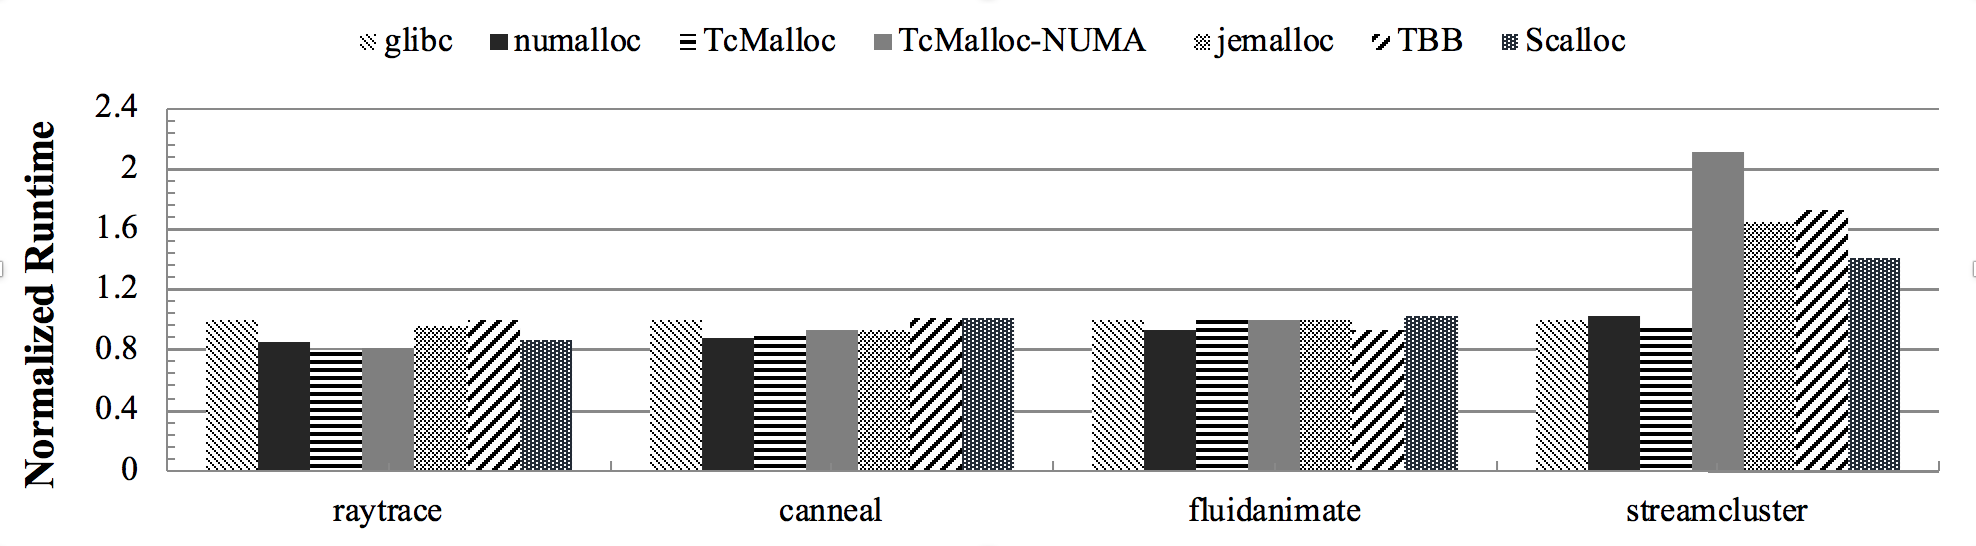
\includegraphics[width=\textwidth,height=150]{figure/2-node-no-interleaved.png}
    \caption{Normalized runtime with different allocators for PARSEC benchmarks in Machine A after shut down interleaved heap}
    \label{2node-parsec-no-interleaved-perf}
\end{figure}

\begin{figure}[H]
    \centering
    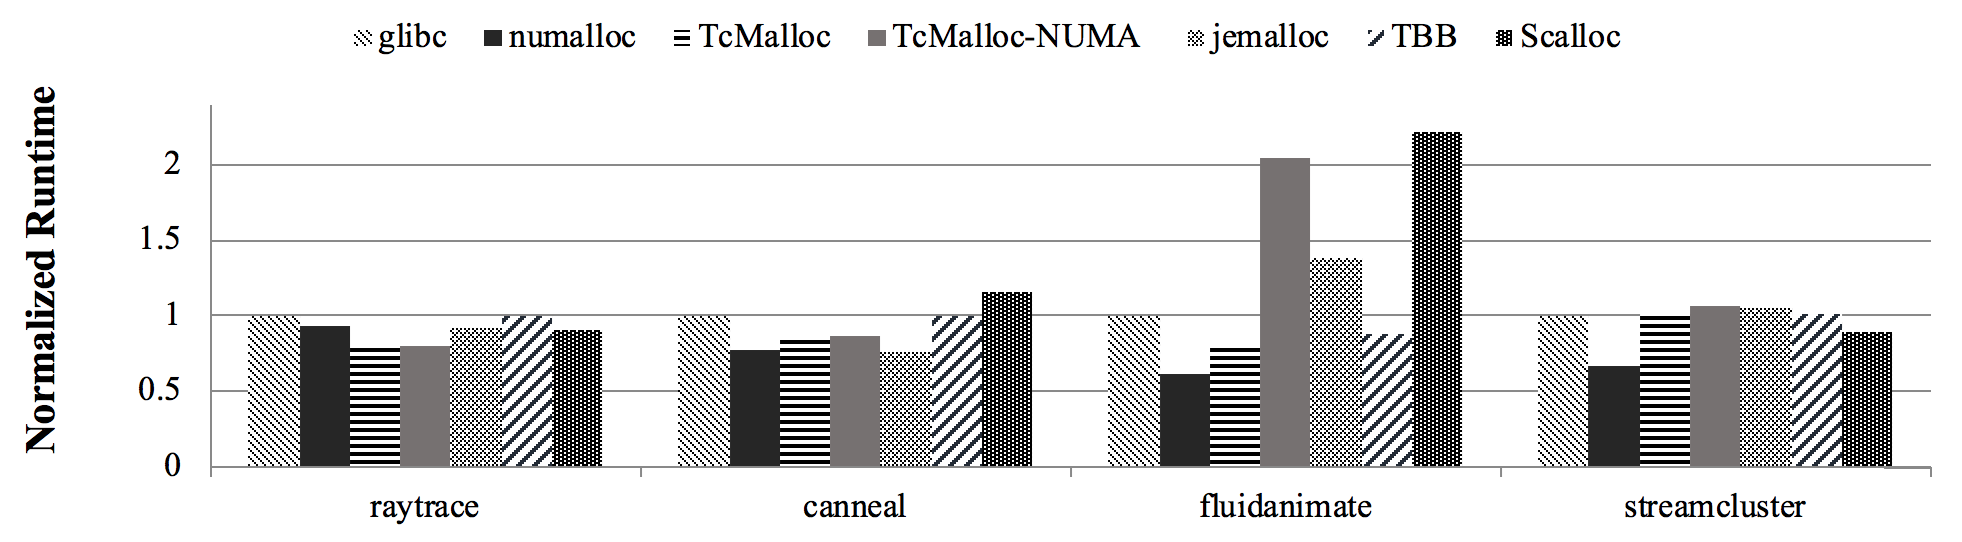
\includegraphics[width=\textwidth,height=150]{figure/8-node-no-interleaved.png}
    \caption{Normalized runtime with different allocators for PARSEC benchmarks in Machine B after shut down interleaved heap}
    \label{8node-parsec-no-interleaved-perf}
\end{figure}
Finally, in figure ~\ref{2node-parsec-no-interleaved-perf} and figure ~\ref{8node-parsec-no-interleaved-perf}, we show some performance results of some applications that got significant different values after we shut down interleaved heap for \NM{}. We can see that for some applicatios with less data sharing between threads like ratrace and canneal, \NM{} could got significant improvements due to its low overheads and proper memory management. But for some other applications with intensive memory operations and sharing like fluidanimate, shutting down interleaved heap could hurt performance, since interleaved heap could help to distributed resource contention evenly over multi-nodes and then got low overheads.

\subsection{Memory Consumption}
\label{sec:memory}

We also measured memory overheads of different allocators for same applications above. For parsec and Hoard benchmarks, the sum of maxresident output from time utility and the size of huge page usage is used,and huge page size could be gotten by periodically collecting /proc/meminfo file. Memory assumption of server applications like MySQL, apache and Memcached is collected by the sum of the VmHWM field and HugetlbPages field from /proc/PID/status file before we shutdownt the server.We always reboot server applications for each single test. 

\begin{figure}[H]
    \centering
    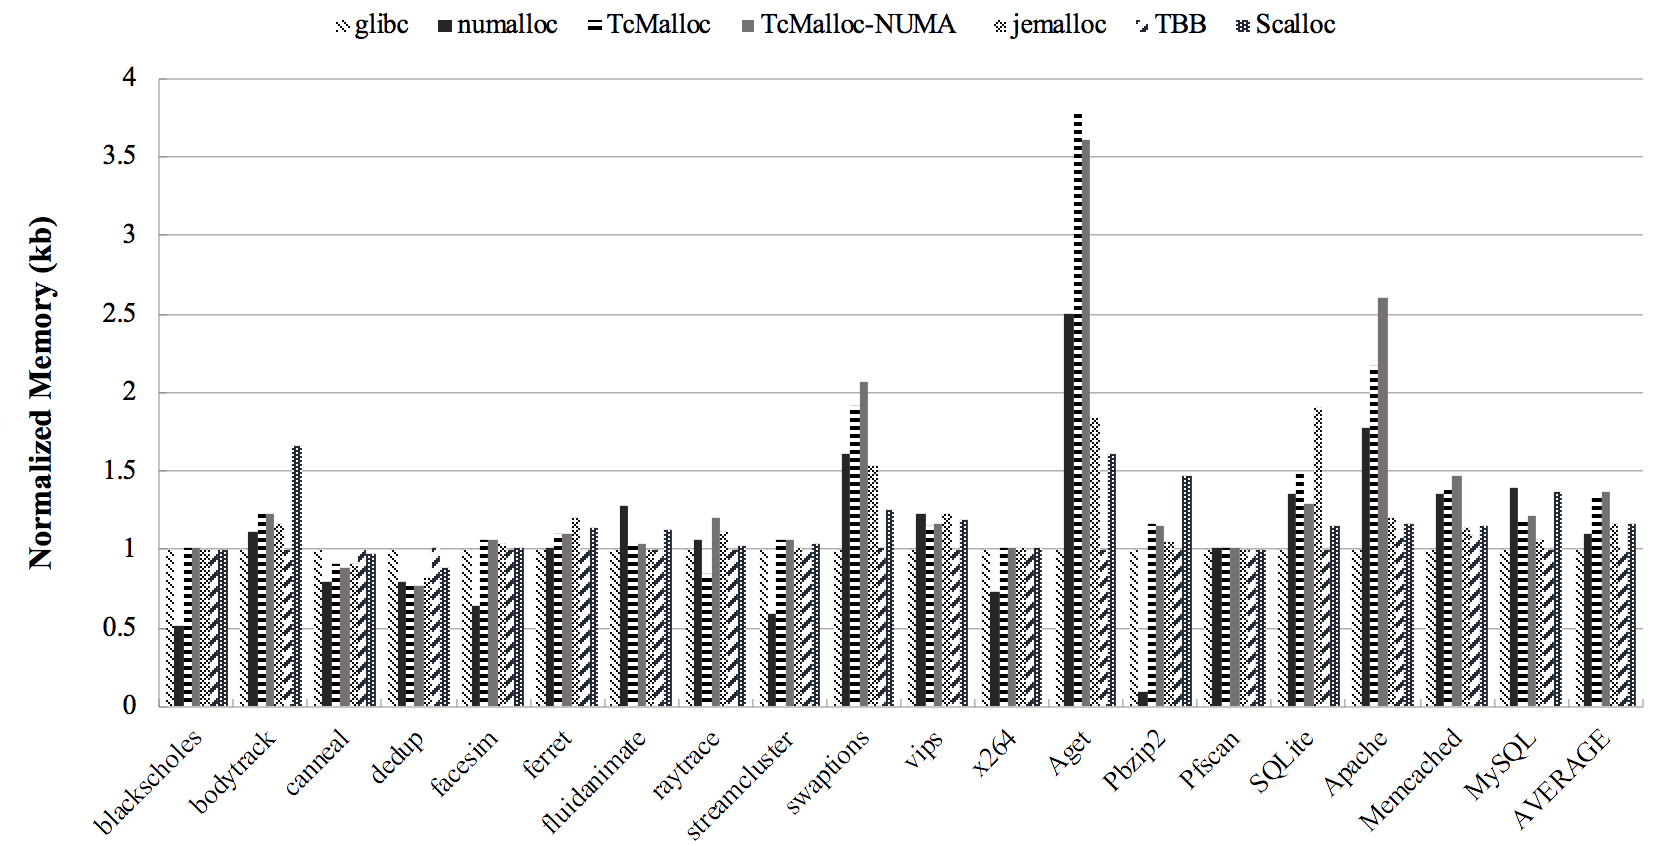
\includegraphics[width=\textwidth,height=200]{figure/2-node-parsec-mem.png}
    \caption{Normalized memory overheads with different allocators for PARSEC benchmarks in Machine A}
    \label{2node-parsec-mem}
\end{figure}

In figure ~\ref{2node-parsec-mem}, we give the normalized memory overheads also compared with Linux's glibc in Machine A. We can see that the average value of \NM{} is 1.09, which means \NM{} costs as same memory as Linux's glibc in average and \NM{} is the best compared with others, although others also do not cost too much. In addition, for most of single application, \NM{} costs as same memory as Linux's glibc or even less like 0.51 for blackscholes and 0.6 for facesim. The most memory consuming application in figure ~\ref{2node-parsec-mem} is Aget ,in which the value of \NM{} is 2.49, but it is still lower than TcMalloc and jemalloc and it is very acceptable. 

\begin{figure}[H]
    \centering
    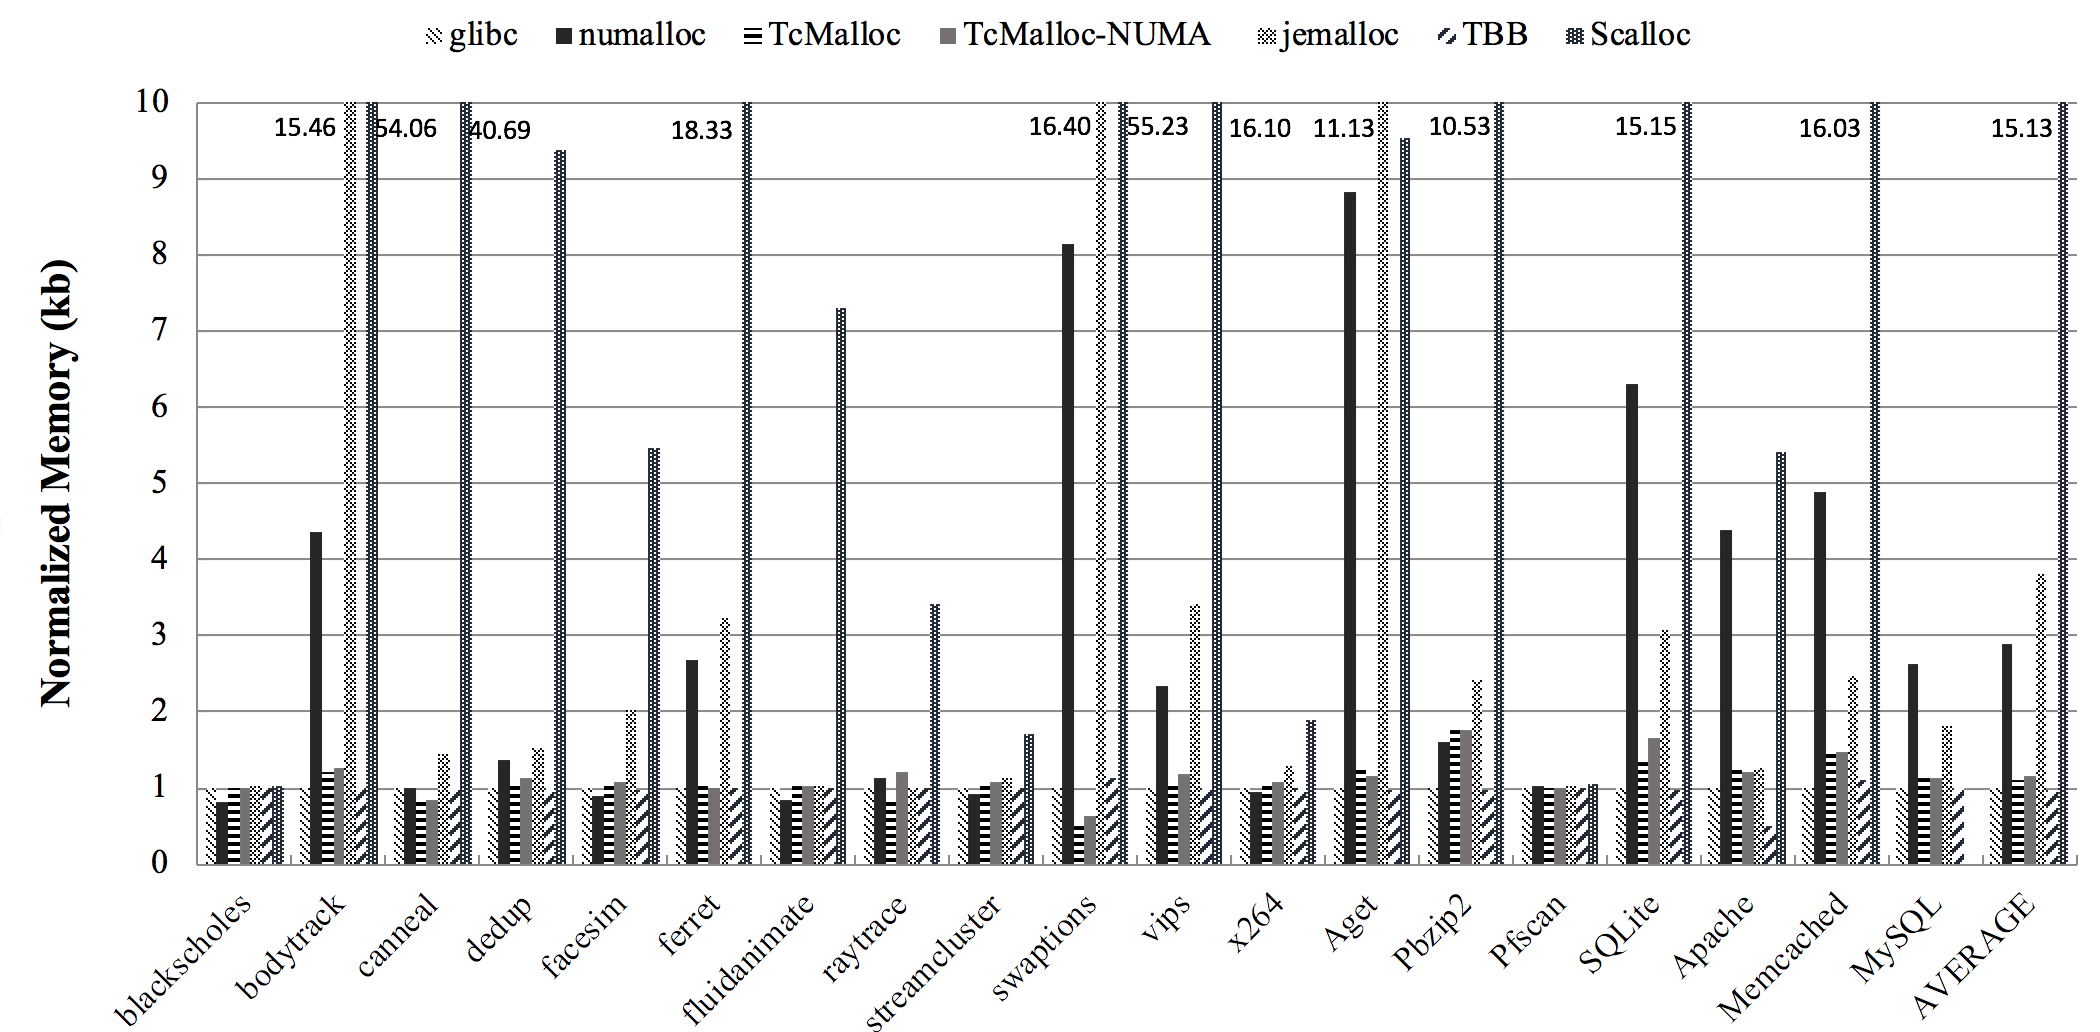
\includegraphics[width=\textwidth,height=200]{figure/8-node-parsec-mem.png}
    \caption{Normalized memory overheads with different allocators for PARSEC benchmarks in Machine B}
    \label{8node-parsec-mem}
\end{figure}

Figure ~\ref{8node-parsec-mem} is the nurmalized memory overheads in Machine B. In this figure, we can see that some allocators get a high average nurmalized value compared with figure ~\ref{2node-parsec-mem}, that \NM{} is 2.9, jemalloc is 3.7 and Scalloc is 15.1. The reason is that there are far more cores in Machine B which is 128 compare with Machine A which is 40. So these allocators will preserve more memories in their thread local area and also per node area in \NM{}, that there are 8 nodes in Machine B and only 2 nodes in Machine A. But we can also see that in most applications like blackscholes, canneal and facesim etc, the memory overheads of \NM{} are actually very low , equal or less than Linux's glibc. Compared with the its huge performance improvements, this memory overheads are negligible.

\begin{figure}[H]
    \centering
    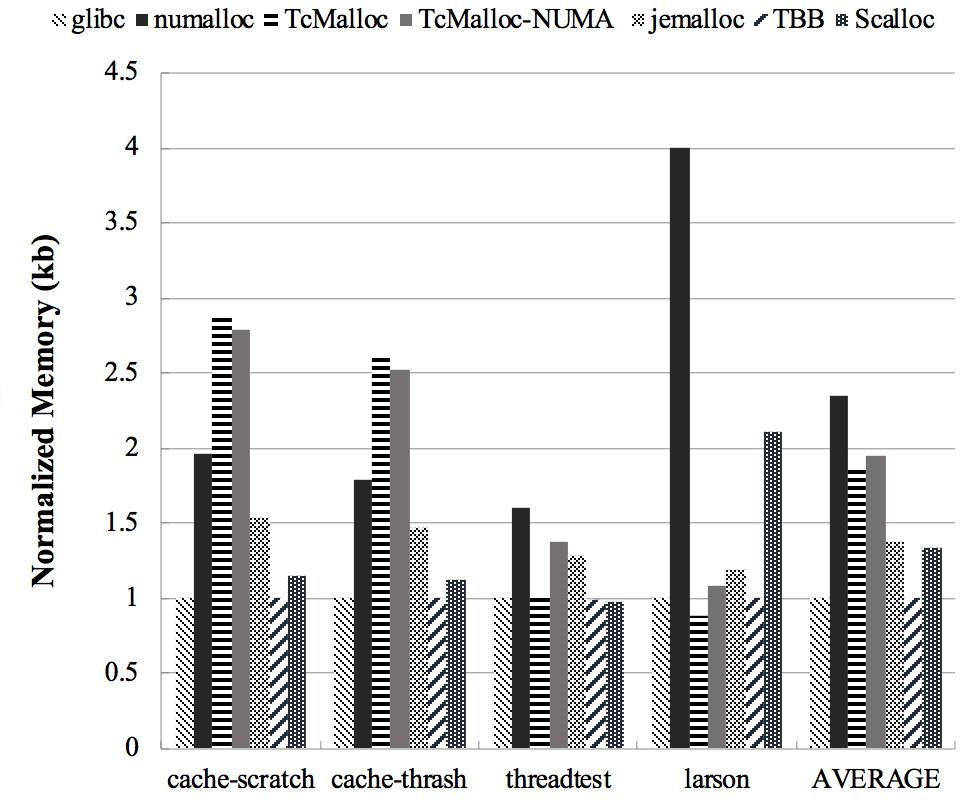
\includegraphics[width=\textwidth,height=200]{figure/2-node-hoard-mem.png}
    \caption{Normalized memory overheads with different allocators for Hoard benchmarks in Machine A}
    \label{2node-hoard-mem}
\end{figure}

\begin{figure}[H]
    \centering
    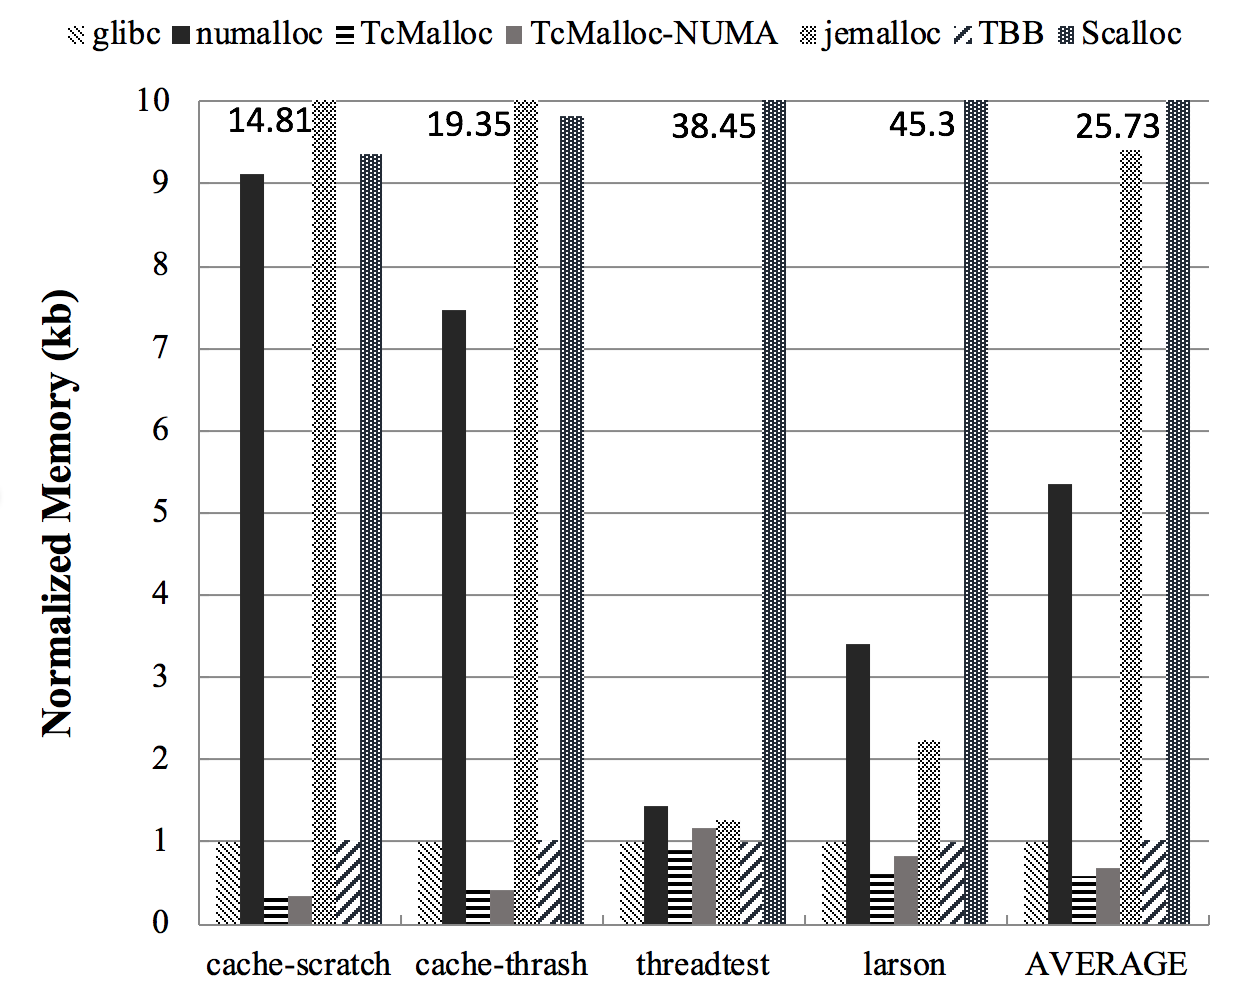
\includegraphics[width=\textwidth,height=200]{figure/8-node-hoard-mem.png}
    \caption{Normalized memory overheads with different allocators for Hoard benchmarks in Machine B}
    \label{8node-hoard-mem}
\end{figure}

Finally, in figure ~\ref{2node-hoard-mem} and ~\ref{8node-hoard-mem}, the normalized memory overheads for Hoard benchmarks are given, and we can see that the average values of all allocators in figure ~\ref{8node-hoard-mem} are bigger than figure ~\ref{2node-hoard-mem}. The reason is same as we mentioned above that there are more cores and more nodes in Machine B than Machine A, so that allocators usually preserve more memories in their thread local area or per node area. In figure ~\ref{2node-hoard-mem}, the average normalized value of \NM{} is larger than others, but actually not too much, which is 2.3 for \NM{}, 1.9 for TcMalloc-NUMA and 1.8 for TcMalloc. It is because that proper node management is utilized in \NM{} and also in TcMalloc-NUMA, so that each node also preserves some memory not only thread locals.But we believe that this little more memory overheads are totally acceptable. It is also the same thing for figure 10, that the average value for \NM{} is little higher than others, which is 5.3. But in this 8 nodes machine, numalloc is not the worst, that Scalloc's average value is 25 and jemalloc is 9.4. One main reason that the value of \NM{} is smaller is that we use mini size bags in \NM{} which is less than the size of one page for small objects and also memories for small objects are shared per node but per cores in Scalloc.

\subsection{Scalability}
\label{sec:scale}
We will evaluate the scalability on 8threads, 16threads, 32 threads, 64 threads and 128 threads. 
(one node, two node, four nodes, and 8 nodes). 

\subsection{Design Choices}
\label{sec:design}

\subsubsection{Interleaved Heap} 

\subsubsection{Thread Binding}
\label{sec: threadbinding}
We will only run it on the 8-node machine. 

